\documentclass[a4paper,12pt,twoside]{report}
\usepackage[left=3.1cm,right=3.1cm,top=2cm,bottom=3cm]{geometry}
%\usepackage[square,authoryear,sort]{natbib}
\usepackage{url}
\usepackage{xcolor}
\usepackage{graphicx}
\usepackage{pdfpages}
\usepackage{subcaption}

\makeatletter
\def\@makechapterhead#1{%
  \vspace*{50\p@}%
  {\parindent \z@ \raggedright \normalfont
    \interlinepenalty\@M
    \Huge\bfseries  \thechapter.\quad #1\par\nobreak
    \vskip 40\p@
  }}
\makeatother

\makeatletter
\newcommand*{\toccontents}{\@starttoc{toc}}
\makeatother


\let\endtitlepage\relax
\begin{document}

\title{\LARGE {\bf PhD Research Proposal:\\Semantic Modelling of Network Traffic for Anomaly Detection}\\
 \vspace*{-5mm}
}
\author{Henry Clausen}
%\date{October 2008}

\maketitle



\toccontents
%\begin{abstract}
%Text
%\end{abstract}



\chapter{Research description}

\section{Introduction and motivation}



Sophisticated data breaches affect hundreds of million customers and inflicts tremendous financial, reputational, and logistic damage. One reason for the recent rise of cyber crime is the increased use of sophisticated techniques for the attack of specific targets. Attackers use customised social engineering and custom-build malware that penetrate defensive barriers and potentially stay undetected in an infected system for an extended period of time. 

Cyber-Security relies on a range of defensive techniques, including sophisticated intrusion detection systems and firewalls that try to detect and prevent attacks against software subsystems. Malicious software still remains the biggest threat to computer users, and its detection is of utmost importance. 


\textcolor{red}{ueberarbeiten******}
Program analysis methods are used widely to automatically test software for particular characteristics and behaviour, and thus identify malicious instances. Close attention has to be paid at the type of features and models that quantify the behaviour of software, as a lack of general program representation leads to low robustness against new or polymorphic malware, and consequently a poor classification performance.  Chen et al.  (2016) \cite{chen2016robust, chen2016more} demonstrated convincingly that semantic features are suitable to reflect the nature of software, benign or malware, in an accurate manner. \textcolor{red}{******ueberarbeiten}

In modern computer networks, it is often impossible to use software analysis on a large-scale basis to prevent network intrusions through malicious software. Here, network intrusion detection systems play a vital role in protecting computer networks from malicious access. The field of intrusion detection is concerned with the development of methods and tools that identify and locate possible intrusions in a computer network. An \textit{intrusion detection system} (IDS) is typically a device or software application that detects malicious activity or policy violations in an automated way by scanning incoming data collected from one or more sources for patterns that a model or a set of rules classifies as malicious.

Intrusion detection is a well researched area, with the first IDSs emerging in the late 1980's. Intrusion detection today comprises a variety of research areas in terms of different types of data sources, system architectures, detection sope, and so forth. Figure \ref{graph} provides a broad yet uncomplete overview of these different areas. 



Current detection methods are predominantly based on the analysis of previously identified attack signatures, which provides great reliability and low false alert rates. However, these methods are dependent on an updated attack signature database and provide no protection against previously unseen attacks. 

Another approach that has recently gained traction in commercial deployment is based on detecting malware and other undesired activity as anomalous behaviour when compared to benign computer activity. In this approach, known as \textbf{traffic anomaly detection}, models that quantify the behaviour of normal network are trained on attack-free traffic data. Observed behaviour that significantly deviates from the trained model is then denoted as anomalous, and the intrusion detection system is taking further steps to investigate a possible intrusion. 



\subsection{Anomaly detection}

Anomaly detection refers to the problem of identifying data instances that have significantly different properties than previously observed \textit{"normal"} data instances. Anomaly detection has its origins in statistical research where normal data instances are assumed to be generated as random variables by a probability distribution $P_\textit{N}(X)$. New data is then identified as anomalous if its properties correspond to regions with vanishing likelihood, i.e. this particular data instance is highly unlikely to be generated by $P_\textit{N}(X)$. The hard part in anomaly detection is normally to use observed data efficiently to build an estimated distribution $\hat{P}_\textit{N}(X)$ that resembles $P_\textit{N}(X)$ closely in order to identify anomalous events while asigning normal instances a non-vanishing likelihood. A variety of techniques exist to achieve this assuming comparibly simple generating distributions. However, this may not always be the case as distributions generating for many interesting types of normal data can be complex and changing over time, and individual data points can have intricate interdependencies. 
\begin{figure}\label{graph}
\centering
\begin{subfigure}[b]{0.45\textwidth}
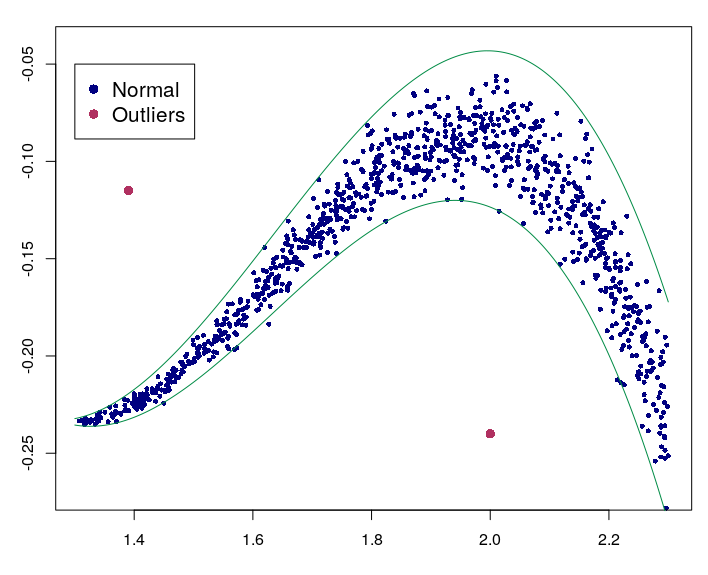
\includegraphics[width=\textwidth]{images/outlier_mine.png}
\caption{}
\end{subfigure}
\begin{subfigure}[b]{0.45\textwidth}
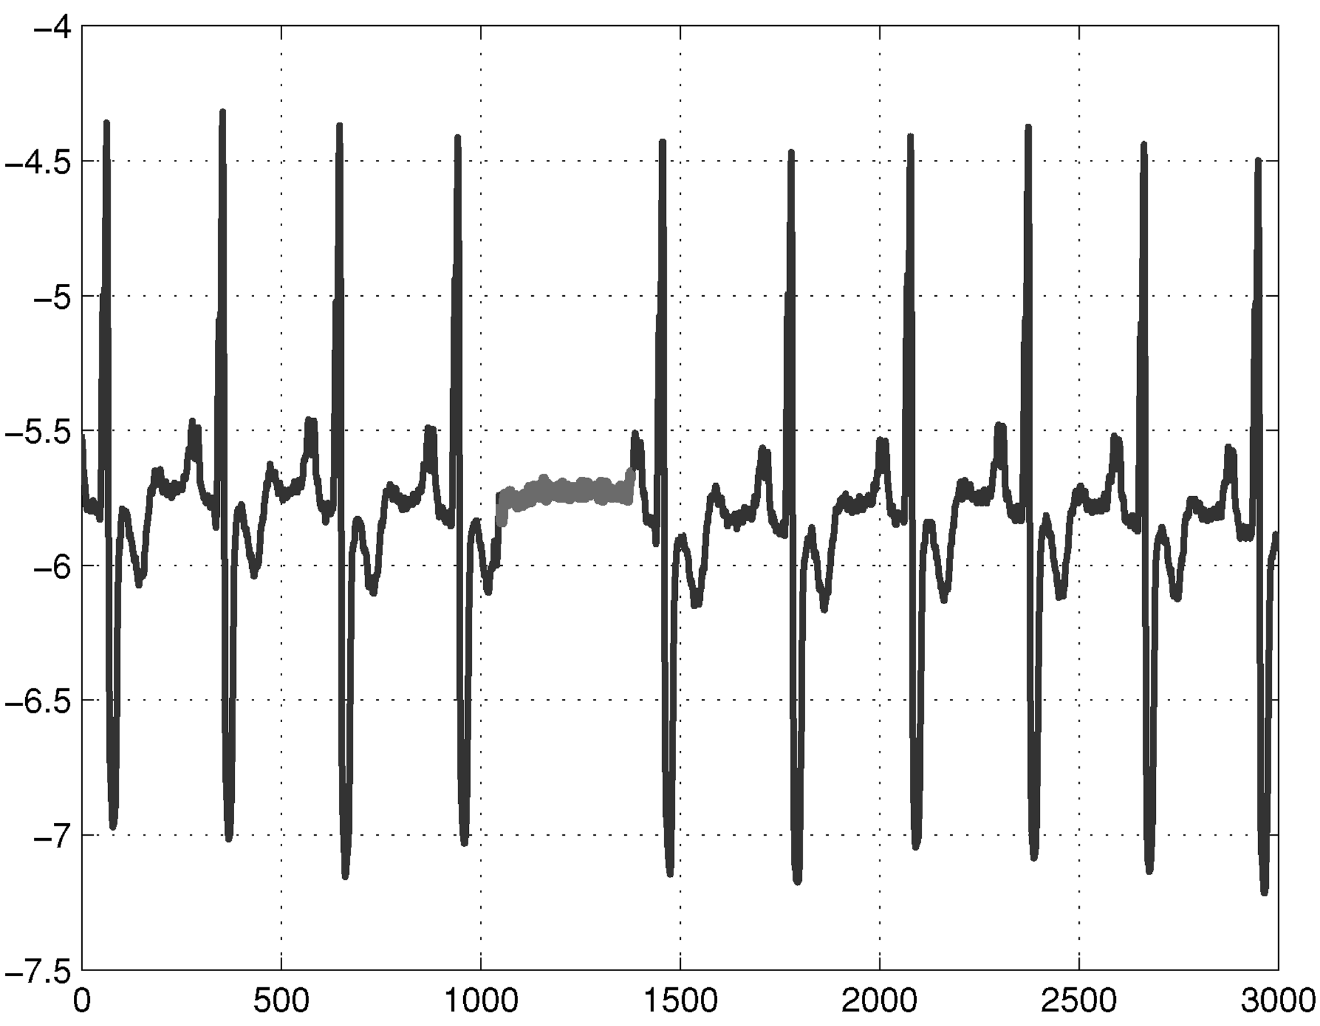
\includegraphics[width=\textwidth]{images/Atrial_Premature_Contraction.png}
\caption{}
\end{subfigure}
\caption{The left plot (a) depicts simple anomalies that deviate in distance from regular data. The right plot (b) shows a contextual anomaly where a group of data instances do not follow a repeating timely behaviour with respect to all other data points (corresponding to an \textit{Atrial Premature Contraction}, taken from \cite{chandola_anomaly_2009})}
\end{figure}

Anomaly detection has found wide application in areas where stability of  critical systems or detection of their abuse is crucial. Examples of these include engine-fault detection in wind-turbines, fraud detection for credit cards. The assumption here is that the modelled system, such as the sensor-data stream of an engine or the buying behaviour of a customer, remains stable and generates consistent data. Detected anomalies in new observations then indicate potential fault or abuse in this system. Obviously, it is not inherently clear that every abuse or fault generates data that differs from normal data. Therefore, it is important to choose data sources are able to reflect the unique nature of a particular system.

\subsubsection{Anomaly detection and NIDS}

Similar to the above described examples, anomaly detection has been applied to network security since the late 90's in order to assist IDSs, with the behaviour of network computers being quantified in the form of events logs capturing network traffic, system calls, etc. The basic approach is to use collected training logs to infer a model of trustworthy activity, and then compare new behaviour against this model. Again, the assumption is that unauthorized and malicious activity will correspond to behaviour that differs from trustworthy one. As an example, an anomalous network traffic pattern in a involving unusual connection pairs could
signify that a hacked computer is extracting or sending out sensitive data to an unauthorized destination.

\textcolor{red}{Insert stuff about NIDS and anomaly detection, drill down on network traffic, maybe talk about technical structure, how training data is gathered, then trained, collection of the traffic, possible anomalies in training data etc, scarcity of datasets. Talk about how anomaly detection should be able to find new attacks compared to signature based approaches}.

\subsubsection{Literature Summary and identified gaps}


Network traffic can be processed into data features of very different nature. Consequently, approaches to apply anomaly detection in network security vary significantly in their scope and methodology. Individual 


Although commercial intrusion detection systems still relies predominantly on \textit{Signature-based} methods, anomaly detection is more and more used  \textcolor{red}{examples}


I provide a detailed analysis of the most important techniques and approaches in my literature review, which can be found in Section \ref{litreview}. 

\chapter{Proposal}

\section{Project aim}

As pointed out above, anomaly detection techniques currently perform best in the detection of attacks of larger volume, such as \textit{DoS attacks} or \textit{Port Scans}, and currently are the most common application in commercial IDS systems \textcolor{red}{reference or example of IDS}. In contrast, research in this area has been less convincing in the context of more targeted attacks that consist of only one or a few connections, with \textit{R2L} and \textit{U2R} attacks currently being the least detected attack classes \cite{nisioti2018intrusion}. 

This can in part be explained by a lack of understanding of how these smaller, more point-like attacks differentiate themselves from normal traffic. Attacks using a larger number of connections will inevitably disturb the  distribution of one or multiple measures of the network, such as the byte-throughput or the port entropy \cite{lakhina2005mining}. However, an attacking connection inserting malicious code to gain control over a computer does not necessarily have different external properties\footnote{also caled \textit{connection summaries}} such as length, size, or port number, than the diverse range of normal connections. Yet, most attempts to detect these attacks via anomaly detection rely exclusively on sumary properties of individual connections or packets to draw a border between normal and malicious traffic.

In this project, I will instead look at the more intrinsic nature of network traffic, the \textit{semantic structure} of packet and connection sequences. \textcolor{red}{argue what that means, why it is promising, and that is has been done before on system calls and promises better robustness}




\section{Work achieved so far}



Significant amount of time has been spent on reflecting on good strategies, data analysis, and appropriate measures to best capture programs distinctinctive signatures. Signatures from Snort have been helpful


\subsection{Alan Turing Data Study Group}


\subsection{Ground truth data generation}

Building semantic models of network traffic means to build an understanding how different network interactions can be distinguished via their traffic trace. We want to use ML techniques to automatically extract meaningful sets of sequences that represent these different interactions. In order to ensure that this is actually true, that our extracted models are indeed representing real, distinguishable interactions and not just nonsense, we need validation from \textit{ground truth data}. 

Network traffic datasets are already hard to obtain due to privacy concerns. However, as  the correspondance between individual network traffic events and their particular purpose are virtually never recorded on a computer, their exist close to zero datasets containing ground truth about the contained events. For that reason, a particular aspect of this project is to generate useful ground truth data with appropriate content myself.

\subsection{Gathering useful data sources}

\subsection{Testing first approaches on realistic data}


\section{Project specific objectives}


\appendix
% appendices come here
\chapter{}
\section{Literature Review}\label{litreview}

%\addcontentsline{toc}{chapter}{Bibliography}
\bibliographystyle{abbrv}
\bibliography{refs}

\end{document}